%; whizzy paragraph -pdf xpdf -latex ./whizzypdfptex.sh
%; whizzy-paragraph "^\\\\begin{frame}"
% latex beamer presentation.
% platex, latex-beamer $B$G%3%s%Q%$%k$9$k$3$H$rA[Dj!#(B

%     Tokyo Debian Meeting resources
%     Copyright (C) 2009 Junichi Uekawa
%     Copyright (C) 2009 Nobuhiro Iwamatsu

%     This program is free software; you can redistribute it and/or modify
%     it under the terms of the GNU General Public License as published by
%     the Free Software Foundation; either version 2 of the License, or
%     (at your option) any later version.

%     This program is distributed in the hope that it will be useful,
%     but WITHOUT ANY WARRANTY; without even the implied warranty of
%     MERCHANTABILITY or FITNESS FOR A PARTICULAR PURPOSE.  See the
%     GNU General Public License for more details.

%     You should have received a copy of the GNU General Public License
%     along with this program; if not, write to the Free Software
%     Foundation, Inc., 51 Franklin St, Fifth Floor, Boston, MA  02110-1301 USA

\documentclass[cjk,dvipdfm,12pt]{beamer}
\usetheme{Tokyo}
\usepackage[english]{babel}
\usepackage{monthlypresentation}

%  preview (shell-command (concat "evince " (replace-regexp-in-string "tex$" "pdf"(buffer-file-name)) "&"))
%  presentation (shell-command (concat "xpdf -fullscreen " (replace-regexp-in-string "tex$" "pdf"(buffer-file-name)) "&"))
%  presentation (shell-command (concat "evince " (replace-regexp-in-string "tex$" "pdf"(buffer-file-name)) "&"))
%  presentation (shell-command (concat "evince " (replace-regexp-in-string "tex$" "pdf"(buffer-file-name)) "&"))

%http://www.naney.org/diki/dk/hyperref.html
%$BF|K\8l(BEUC$B7O4D6-$N;~(B
\AtBeginDvi{\special{pdf:tounicode EUC-UCS2}}
%$B%7%U%H(BJIS$B7O4D6-$N;~(B
%\AtBeginDvi{\special{pdf:tounicode 90ms-RKSJ-UCS2}}

\newenvironment{commandline0}%
{\VerbatimEnvironment
  \begin{Sbox}\begin{minipage}{0.95\hsize}\begin{fontsize}{9}{9} \begin{BVerbatim}}%
{\end{BVerbatim}\end{fontsize}\end{minipage}\end{Sbox}
  \setlength{\fboxsep}{10pt}

\vspace{10pt}% skip before
\fcolorbox{dancerdarkblue}{dancerlightblue}{\TheSbox}

\vspace{6pt}% skip after
}
%end of commandline

\title{$BEl5~%(%j%"(B Debian $BJY6/2q(B}
\subtitle{Linux$B%+!<%M%k%3%s%U%#%0JQ49%D!<%k(B\\$B$r:n$C$F$_$?(B}
\author{$B4d>>(B $B?.MN(B iwamatsu@debian.or.jp\\IRC nick: iwamatsu}
\date{2009$BG/(B1$B7n(B17$BF|(B}
\logo{
\includegraphics[width=8cm]{image200607/openlogo-light.eps}}

\begin{document}

\frame{\titlepage{}}


\emtext{$BE_5Y$_(B}
\section{$B@V$A$c$s$,@8$^$l$^$7$?(B}
\begin{frame}[containsverbatim]{$B@V$A$c$s$,@8$^$l$^$7$?(B}
$B@V$A$c$s$,@8$^$l$?$N$G!"@$OC$r$7$F$$$^$7$?!#(B
 \begin{center}
 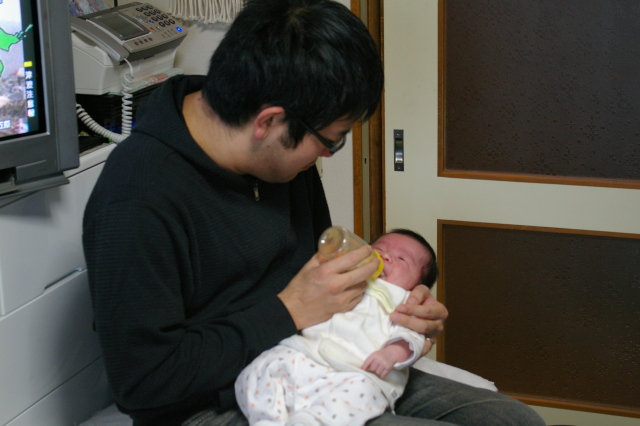
\includegraphics[scale=0.5]{image200901/baby.jpg}
 \label{fig:baby}
 \end{center}
\end{frame}

\emtext{$B:#2s:n$C$?$b$N(B}
\section{$B:#2s:n$C$?$b$N(B}
\begin{frame}[containsverbatim]{$B:#2s:n$C$?$b$N(B}
\begin{center}\bfseries
$B%7%9%F%`>pJs$r85$K(B\\
$B%7%9%F%`$KI,MW$J%+!<%M%k%b%8%e!<%k$r(B\\
$BAH$_9~$_;XDj$KJQ49$7$?(B\\
$B%+!<%M%k%3%s%U%#%0%U%!%$%k$r=PNO$9$k(B\\
$B%9%/%j%W%H(B
\end{center}
\end{frame}
\begin{frame}[containsverbatim]{$B:#2s:n$C$?$b$N(B}
\begin{center}
$B$?$$$7$F$b$N$G$O$J$$$G$9(B
\end{center}
\end{frame}


\begin{frame}{$B$J$<$3$l$r:n$m$&$H;W$C$?$N$+(B}
\begin{enumerate}
\item $B$R$5$S$5$K$"$^$j;H$C$F$J$$%^%7%s$N%+!<%M%k%3%s%U%#%0%l!<%7%g%s$r$7$?!#(B
\item $B%3%s%U%#%0%l!<%7%g%s$,B?$9$.$k!#(B
\item $BFC$K(BPC$B$@$H2?$r;XDj$7$F$$$$$b$N$d$i!#(B
\item $B<+F02=$G$-$k$s$8$c$M!)(B
\item $B<+J,$O@55,I=8=$,6l<j!#@55,I=8=$NJY6/$N$?$a!#(B
\item Perl$B$r3X=,$9$kI,MW$,$"$C$?!#(B
\item $B$3$l$i$,$G$-$F!"%"%&%H%W%C%H$N$G$-$k$b$N$r:n$j$^$9$+!#(B
\item $B5">J$N?744@~Fb$G!#(B
\end{enumerate}
\end{frame}

\begin{frame}{$B$3$l$,$G$-$k$H(B}
\begin{enumerate}
\item $B%+!<%M%k%3%s%U%#%0$KG:$^$5$l$:$K$9$`(B
\item $B<h$j9g$($:F0$/%+!<%M%k$O$G$-$k!J$O$:!K(B
\item $B0lHL%f!<%6$+$i(Bvanila$B%+!<%M%k%"%/%;%9$X$NI_5o$,2<$,$k!J$+$b!K(B
\end{enumerate}
\end{frame}

\section{$B$J$<H`$i$O%+!<%M%k$r%j%3%s%Q%$%k$9$k$N$+!)(B}
\begin{frame}[containsverbatim]{}
\begin{center}
\large\bfseries
$B$=$&$$$d!"%+!<%M%k%3%s%Q%$%k!*%3%s%Q%$%k!*$C$F$&$k$5$$?M$?$A$$$k$h$M!)(B
\end{center}
\end{frame}

\begin{frame}[containsverbatim]
\begin{center}
\large\bfseries
$B$J$<H`$i$O%+!<%M%k$r%j%3%s%Q%$%k$9$k$N$+!)(B
\end{center}
\end{frame}

\begin{frame}{$B%+!<%M%k$r%j%3%s%Q%$%k$9$kM}M3(B}
\begin{itemize}
\item $B%+!<%M%k%O%C%/$N$?$a!#(B
\item $B%+!<%M%k(BBTS$B$N?<DI$$!#(B
\item $B:G?7$N%+!<%M%k$O?7$7$$%I%i%$%P$d5!G=$,;H$($k$+$i!#(B
\item $B%I%i%$%P$rAH$_9~$_$K$7$F!"5/F0$N9bB.2=!#(B
\item $B%I%-%I%-46$rL#$o$&$3$H$,$G$-$k!#(B
\item $BL5BL$K(BCPU$B$r;H$$$?$$!#(B($BH?%(%3(B)
\end{itemize}
\end{frame}

\begin{frame}{$B%+!<%M%k$r%j%3%s%Q%$%k$9$k$3$H$K$h$k%G%a%j%C%H(B}
\begin{itemize}
\item $B<:GT$7$?$iF0$+$J$/$J$k$+$b$7$l$J$$!#(B
\item $B%3%s%Q%$%k$K(BCPU$B%j%=!<%9$r?)$$$9$.$k(B(CPU$B$,CY$$$?$a(B)$B!#(B
\end{itemize}
\end{frame}

\begin{frame}{$B$J$<H`$i$O%+!<%M%k$r%j%3%s%Q%$%k$9$k$N$+!)(B}
\begin{center}
\large\bfseries
$B$3$3$K$$$k$R$H$?$A$K$O(B\\
$B8e<T$J$s$F5$$K$7$J$$$H;W$$$^$9$,!#(B
\end{center}
\end{frame}

\emtext{$BFbMF(B}

\begin{frame}[containsverbatim]{$BI,MW$J%G!<%?(B}

\begin{itemize}
\item $B;H$&%+!<%M%k(B\\
      Debian$B$GDs6!$7$F$$$k%+!<%M%k(B(lenny $B$G$O(B 2.6.26)
\item $BF~NO$9$k%G!<%?(B
\begin{enumerate}
  \item $B%+!<%M%k%=!<%9%3!<%I(B
  \item $BF0$$$F$$$k%+!<%M%k$N%3%s%U%#%0%U%!%$%k(B\\
	\url{/boot/config-2.6.26-1-xxx}
  \item $B%7%9%F%`>pJs(B
\end{enumerate}
\item $B=PNO$5$l$k%G!<%?(B\\
      $B%7%9%F%`>pJs$r85$K%7%9%F%`$KI,MW$J%+!<%M%k%b%8%e!<%k$,AH$_9~$_(B
      $B>uBV$K$J$C$F$$$k%+!<%M%k%3%s%U%#%0%U%!%$%k(B
\end{itemize}
\end{frame}


\subsection{$B%7%9%F%`>pJs$N<hF@J}K!(B}
\begin{frame}[containsverbatim]{$B%7%9%F%`>pJs$N<hF@J}K!(B}
$B$I$N$h$&$K$7$F!"%7%9%F%`>pJs$r<hF@$9$k$+!#(B

\begin{table}[h]
 \begin{center}
 {
   \begin{tabular}{l|l} \hline
     $B%3%^%s%I(B & $BFbMF(B  \\ \hline \hline
     dmidecode & BIOS $B$+$i%7%9%F%`>pJs$r=PNO$9$k(B \\
     lspci & PCI $B$N>pJs$r=PNO$9$k(B \\
     lsusb & USB $B$N>pJs$r=PNO$9$k(B \\
     dmesg & $B%+!<%M%k%G%P%C%0%a%C%;!<%8$r=PNO$9$k(B \\
     lsmod & $B%m!<%I$7$F$k%b%8%e!<%k$r=PNO$9$k(B \\
   \end{tabular}
 }
 \caption{$B5/F0$7$F$$$k%+!<%M%k$+$iF@$i$l$k>pJs(B}
 \label{kernel-output}
 \end{center}
\end{table}

\end{frame}

\subsection{$B%7%9%F%`>pJs$N<hF@J}K!(B}
\begin{frame}[containsverbatim]{$B%7%9%F%`>pJs$N<hF@J}K!(B}

$B:#2sMxMQ$7$?$b$N(B

\begin{table}[h]
 \begin{center}
 {
   \begin{tabular}{l|l} \hline
     $B%3%^%s%I(B & $BFbMF(B  \\ \hline \hline
     lsmod & $B%m!<%I$7$F$k%b%8%e!<%k$r=PNO$9$k(B \\
   \end{tabular}
 }
 \caption{$B5/F0$7$F$$$k%+!<%M%k$+$iF@$i$l$k>pJs(B}
 \label{kernel-output}
 \end{center}
\end{table}


{\bf $B%m!<%I$7$F$$$k%b%8%e!<%k!a8=:_$N(B Linux $B%7%9%F%`$KI,MW$J$b$N(B}
$B$J$N$G!"$o$+$j$d$9$$!#(B
\end{frame}

\emtext{$B4JC1$JN.$l(B}

\begin{frame}{$B4JC1$JN.$l(B}
1. $B%G!<%?$H$7$F!"(B
\begin{enumerate}
\item $B%+!<%M%k%=!<%9%3!<%I$X$N%Q%9(B
\item $BF0:n$7$F$$$k%+!<%M%k%3%s%U%#%0%U%!%$%k(B
\item lsmod $B$N=PNO7k2L(B
\end{enumerate}
$B$r;XDj$9$k!#(B

\end{frame}

\begin{frame}[containsverbatim]{$B4JC1$JN.$l(B}
2. lsmod $B$+$i%m!<%I$7$F$$$k%I%i%$%P%b%8%e!<%k0lMw$r<hF@$9$k(B

lsmod $B$r<B9T$9$k$H!"0J2<$N$h$&$JFbMF$,=PNO$5$l$k!#(B
\begin{commandline0}
$ lsmod
Module                  Size  Used by
i915                   25280  2
drm                    65256  3 i915
ipv6                  235300  10
rfcomm                 28272  2
l2cap                  17248  9 rfcomm
........
\end{commandline0}
\end{frame}

\begin{frame}[containsverbatim]{$B4JC1$JN.$l(B}

{\bf 3. $B%I%i%$%P%b%8%e!<%kL>(B $B$H(B modinfo $B%3%^%s%I$+$i(B $B%I%i%$%P%b%8%e!<%k$N%Q%9$r<hF@$9$k!#(B}
\\

modinfo $B%3%^%s%I$r;H$&$H!";XDj$7$?%I%i%$%P%b%8%e!<%kL>$N>pJs$r<hF@$9$k$3(B
       $B$H$,$G$-$^$9!#(B-n $B%*%W%7%g%s$r;H$&$H!"%I%i%$%P%*%V%8%'%/%H%U%!%$%k(B
       $B$N%Q%9$,=PNO$5$l$k!#(B

\begin{commandline0}
$ modinfo -n i915
/lib/modules/2.6.26-1-amd64/kernel/drivers/char/drm/i915.ko
\end{commandline0}
\end{frame}

\begin{frame}[containsverbatim]{$B4JC1$JN.$l(B}
\begin{commandline0}
$ modinfo -n i915
/lib/modules/2.6.26-1-amd64/kernel/drivers/char/drm/i915.ko
\end{commandline0}
 $B>e$N7k2L$rNc$K$9$k$H!"(B{\bf /lib/modules/2.6.26-1-amd64/kernel/} $B0J2<$H(B $B%+!<%M%k%=!<%9(B
 $B%3!<%I$N%Q%99=B$$OF1$8$J$?$a!"%I%i%$%P%b%8%e!<%kL>(B{\bf i915}$B$N(B Makefile
 $B$N$"$k%Q%9$O(B {\bf drivers/char/drm/Makefile} $B$K$J$k!#(B

$B$^$?!"%I%i%$%P%*%V%8%'%/%H%U%!%$%k$O(B {\bf i915.ko} $B$G$"$k$3$H$,J,$+$k!#(B
\end{frame}


\begin{frame}[containsverbatim]{$B4JC1$JN.$l(B}

{\bf 4. $B@h$G<hF@$7$?(BMakefile $B$X$N%Q%9$H%I%i%$%P%*%V%8%'%/%H%U%!%$%kL>$h$j!"(B
      $BBP>]$K$J$k%I%i%$%P%3%s%U%#%0L>$r<hF@$9$k!#(B}

      $B%I%i%$%P%*%V%8%'%/%H%U%!%$%k(B(i915.ko)$B$H%I%i%$%P%b%8%e!<%kL>(B(i915)
      $B$OI,$:$7$b0lCW$9$k$H$O8B$i$J$$$N$G!"%I%i%$%P%b%8%e!<%kL>$r;H$C$F!"(B
      $B%I%i%$%P%3%s%U%#%0L>$r8!:w$9$k!#(B($BNc$($P(B snd\_hda\_intel)

\begin{commandline0}
.....
obj-$(CONFIG_DRM_I830)  += i830.o
obj-$(CONFIG_DRM_I915)  += i915.o <- $B$3$l(B
obj-$(CONFIG_DRM_SIS)   += sis.o
.....
\end{commandline0}
\end{frame}

\begin{frame}[containsverbatim]{$B4JC1$JN.$l(B}

{\bf 5. $B<hF@$7$?%I%i%$%P%3%s%U%#%0L>$rJ]B8$9$k!#(B}
\end{frame}

\begin{frame}[containsverbatim]{$B4JC1$JN.$l(B}

{\bf 6. $BF0:n$7$F$$$k%+!<%M%k%3%s%U%#%0%U%!%$%k$N%I%i%$%P%3%s%U%#%0$r=q$-49$($k!#(B}

$B@55,I=8=$r;H$C$F=q$-49$($k$H!"0J2<$N$h$&$K$J$k!#(B
{\bf m} $B$O%b%8%e!<%k$r0UL#$7!"(B{\bf y} $B$OAH$_9~$_$r0UL#$9$k!#(B

$BJQ99A0(B
\begin{commandline0}
....
CONFIG_DRM_I830=m
CONFIG_DRM_I915=m
CONFIG_DRM_MGA=m
....
\end{commandline0}

$BJQ998e(B
\begin{commandline0}
....
CONFIG_DRM_I830=m
CONFIG_DRM_I915=y <- $B=q$-49$((B
CONFIG_DRM_MGA=m
....
\end{commandline0}
\end{frame}

\begin{frame}[containsverbatim]{$B4JC1$JN.$l(B}

{\bf 7. $BJQ99$7$?$b$N$r%U%!%$%k$K=PNO$9$k!#(B}

\end{frame}


\emtext{$B<B:]$K;H$C$F$_$k(B}

\begin{frame}[containsverbatim]{ $B<B:]$K;H$C$F$_$k(B}
\begin{commandline0}
$ moge -h
moge - Script to Kernel Module Enabler from lsmod command output

Copyright (C) 2008,2009 Nobuhiro Iwamatsu <iwamatsu@nigauri.org>
Usage: moge [options]
	-c, --configfile <file>   Kernel config file name
	-k, --kernel              Kernel source path
	-o, --output <file>       outout file
	-l, --lsmod               lsmod command output file
	-h, --help                display this help screen and exit
	-v, --version             show the version and exit

By Nobuhiro Iwamatsu <iwmatsu@nigauri.org>
$ moge -o sage -c config-2.6.26-1-686 -l lsmod.list -k \
                         /usr/src/linux-2.6-2.6.26/
\end{commandline0}
\end{frame}


\emtext{$B:n@.$5$l$?%3%s%U%#%0%U%!%$%k$r;H$C$F%+!<%M%k$r%3%s%Q%$%k$9$k(B}

\begin{frame}[containsverbatim]{$B%+!<%M%k%3%s%Q%$%k$r$9$k(B}
$B:n@.$5$l$?%3%s%U%#%0%U%!%$%k$r;H$C$F%+!<%M%k$r%3%s%Q%$%k$7$F$_$k!#(B

\begin{commandline0}
$ sudo apt-get update
$ sudo apt-get install linux-source-2.6.26 kernel-package
$ cd /usr/src/linux-source-2.6.26
$ make oldconfig
$ fakeroot make-kpkg --revision=yourpc00 kernel_image kenrel_header
$ ls ../
linux-image-2.6.26_yourpc00_i386.deb
linux-headers-2.6.26_yourpc00_i386.deb
.......
\end{commandline0}
\end{frame}

\section{$BJQ997k2L(B}
\begin{frame}[containsverbatim]{lsmod$B$N7k2L(B}

eeePC $B$G;n$7$F$_$F!"$I$l$0$i$$JQ$o$C$?$N$+D4$Y$F$_$?!#(B

$BJQ99A0(B 61$B%b%8%e!<%k(B
\begin{commandline0}
$ lsmod
Module                  Size  Used by
i915                   25280  2
drm                    65256  3 i915
ipv6                  235300  10
rfcomm                 28272  2

......

ide_core               96168  1 ide_pci_generic
ehci_hcd               28428  0
uhci_hcd               18672  0
usbcore               118160  5 uvcvideo,usb_storage,ehci_hcd,
uhci_hcd
thermal                15228  0
processor              32576  2 thermal
fan                     4164  0
thermal_sys            10856  4 video,thermal,processor,fan
\end{commandline0}
\end{frame}

\begin{frame}[containsverbatim]{lsmod$B$N7k2L(B}

 $BJQ998e(B 0$B%b%8%e!<%k(B
\begin{commandline0}
$ lsmod
Module                  Size  Used by
\end{commandline0}

\end{frame}

\begin{frame}{bootchart}

{\bf bootchart$B$G$I$l$0$i$$5/F0$,B.$/$J$C$?$+!"D4$Y$F$_$^$7$?!#(B}

\end{frame}

\begin{frame}{bootchart $BJQ99A0(B}
\begin{figure}
 \begin{center}
 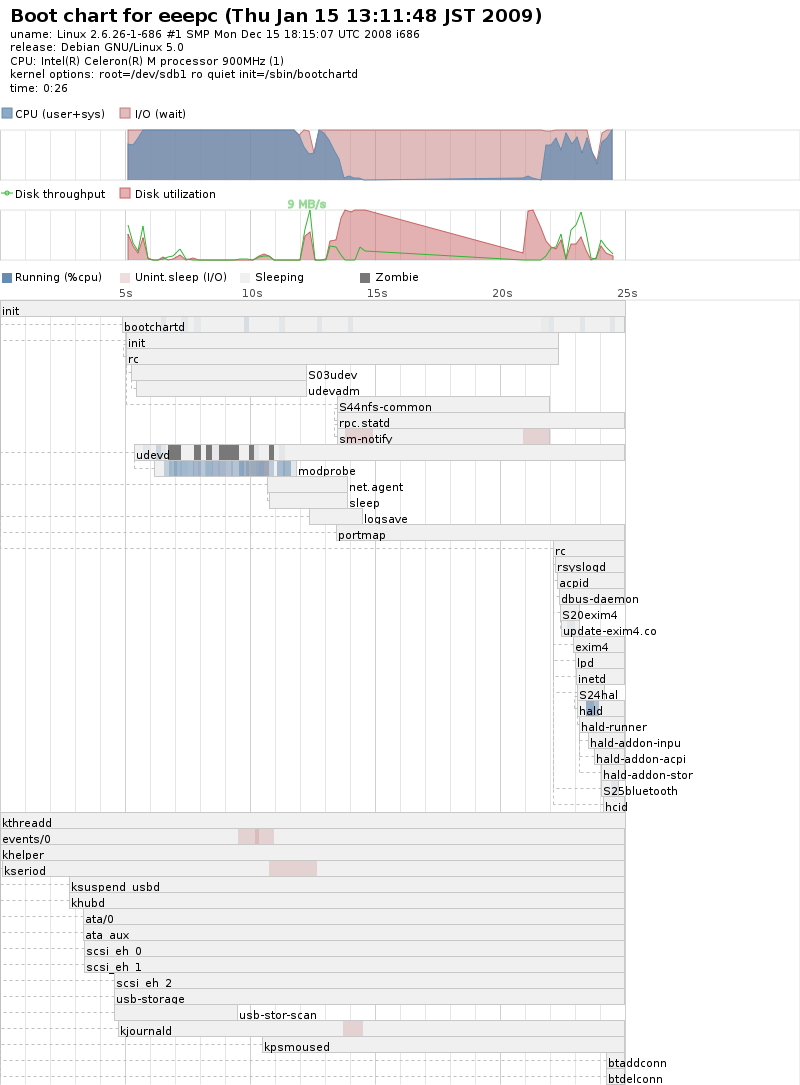
\includegraphics[scale=1.0]{image200901/bootchart-eeepc.png}
 \caption{$BJQ99A0$N(Bbootchart}
 \label{fig:bootchart-eeepc}
 \end{center}
\end{figure}

\end{frame}

\begin{frame}{bootchart $BJQ998e(B}
\begin{figure}
 \begin{center}
 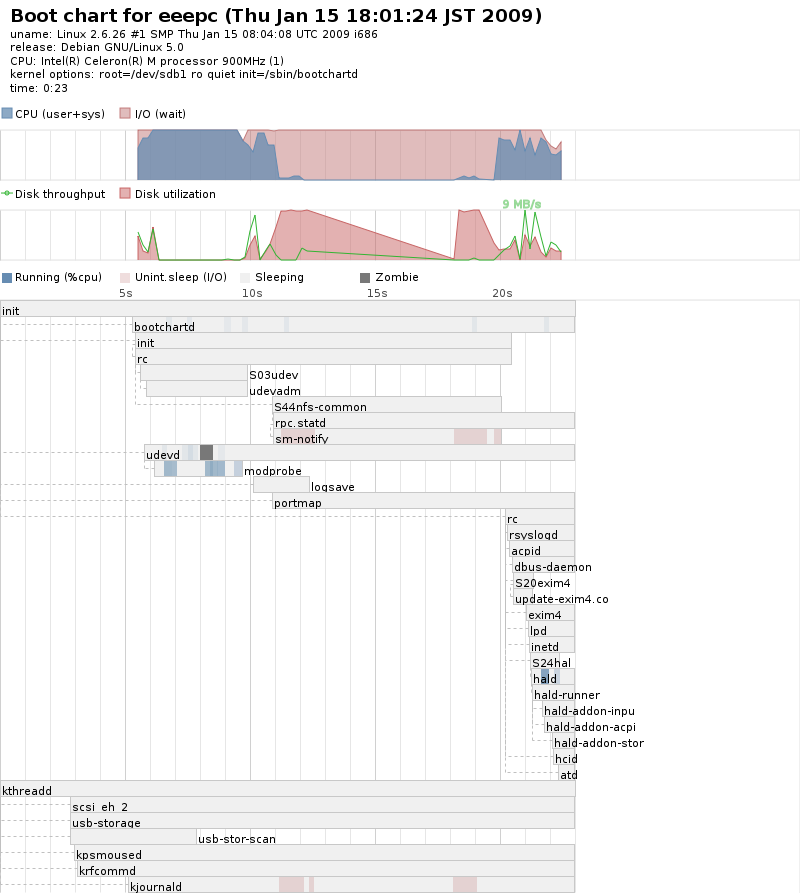
\includegraphics[scale=1.0]{image200901/bootchart-eeepc-new.png}
 \caption{$BJQ998e$N(Bbootchart}
 \label{fig:bootchart-eeepc-new}
 \end{center}
\end{figure}

\end{frame}

\begin{frame}{$B%b%8%e!<%k%m!<%IItJ,(B}
\begin{figure}
 \begin{center}
 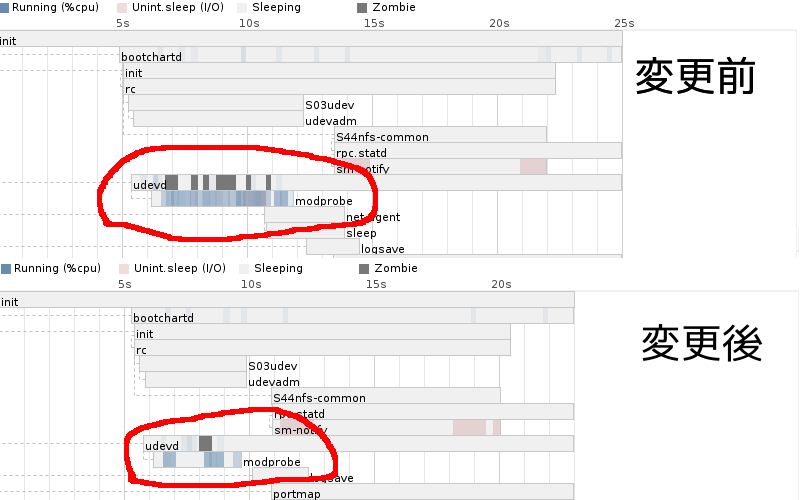
\includegraphics[scale=0.6]{image200901/bootchart-eeepc-merge.png}
 \caption{$B%b%8%e!<%k%m!<%IItJ,(B}
 \label{fig:bootchart-eeepc-merge}
 \end{center}
\end{figure}

\end{frame}


\section{$B:#8e$NM=Dj(B}
\begin{frame}{$B:#8e$NM=Dj(B}
\begin{enumerate}
 \item make-kpkg $B$KF~$l$k!)(B
 \item $B%Q%C%1!<%82=!)(B
 \item $B%+!<%M%k%3%s%Q%$%k(BWeb$B%5!<%S%9$NDs6!!)(B
 \item $B%I%i%$%P%*%V%8%'%/%H%U%!%$%k$H%I%i%$%P%b%8%e!<%kL>$,0lCW$7$J$$$d$D$rD>$9!#(B
\end{enumerate}
\end{frame}


\end{document}

%;;; Local Variables: ***
%;;; outline-regexp: "\\([ 	]*\\\\\\(documentstyle\\|documentclass\\|emtext\\|section\\|begin{frame}\\)\\*?[ 	]*[[{]\\|[]+\\)" ***
%;;; End: ***
